\lab{Applications}{Regression}{Regression}
\label{Stats3?}

\objective{This section will introduce the very basics of Linear Regression (both simple and multiple) and Logistic Regression.}
Dependencies: Least squares

\section*{Introduction to Linear Regression}

One of the first skills in taught in basic algebra is to effectively plot the line $y=mx+b$.  But what if we want to find the line that best fits points?

\begin{figure}[h]
\centering
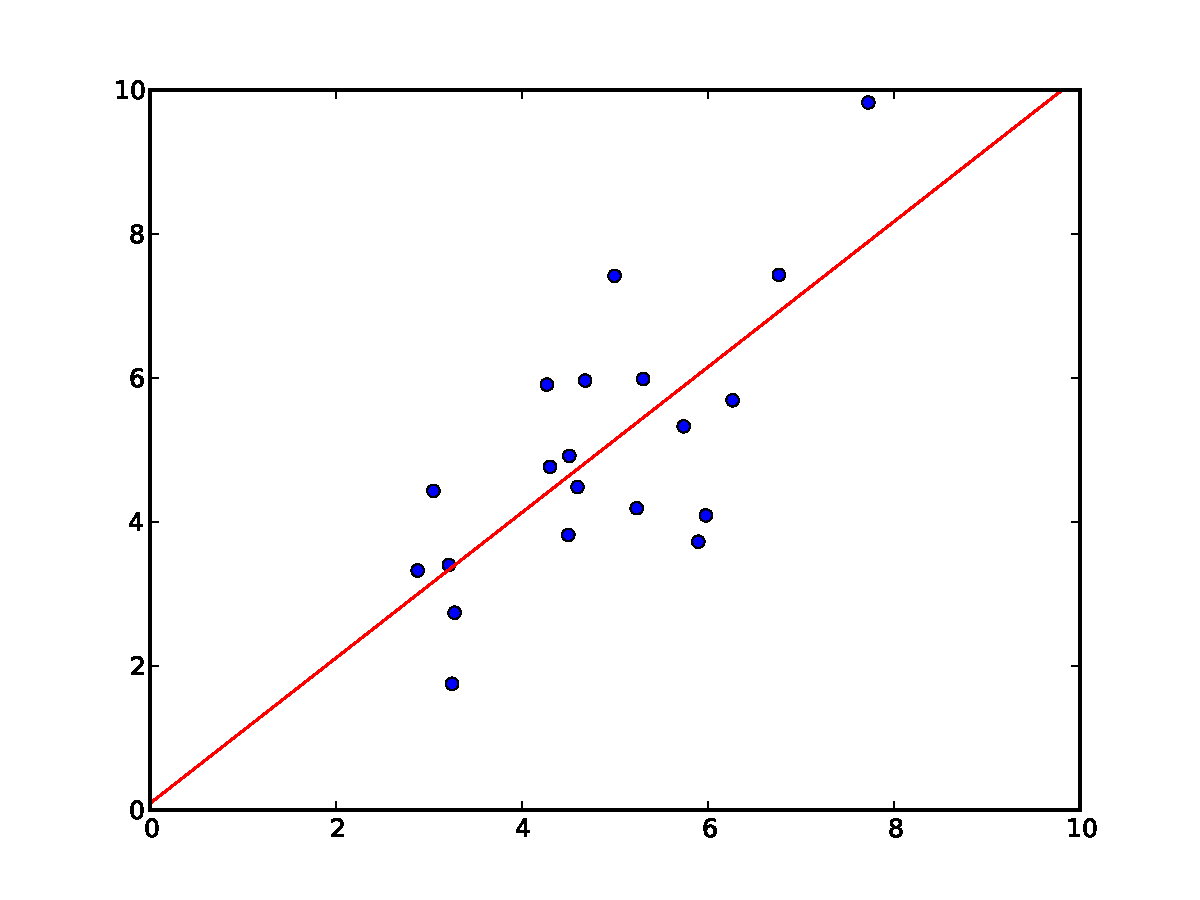
\includegraphics[width=3in]{slr.pdf}
\end{figure}

Here, we can use ordinary least squares. If the line is $y=mx+b$, then let $$y_i = mx_i + b +\epsilon_i$$ describe point $i$, $i \in \{1,...,n\}$, where $\epsilon_i$ is vertical distance from the point to the line, and is often called the residual or the error. These equations for all $n$ points can be described in vector notation. Let the different coordinates of the points be represented by a column vector $\underline{x}$ and a column vector $\underline{y}$, each of length n. Note that all vectors in this section will be assumed to be column vectors unless otherwise noted. Then $$\underline{y}=m\underline{x}+b\underline{1}+\underline{\epsilon} = (\underline{1}, \underline{x}) \begin{pmatrix} b \\ m \end{pmatrix} + \underline{\epsilon}.$$ 

In statistical science, the intercept and slope ($b$ and $m$) are called coefficients and denoted as $\beta_0$ and $\beta_1$ respectively, where $\begin{pmatrix} \beta_0 \\ \beta_1 \end{pmatrix} = \underline{\beta}$. Also, we will denote $(\underline{1}, \underline{x})$ as $X$. Thusly, our equation now reads as $$\underline{y}=X\underline{\beta}+\underline{\epsilon}.$$ This notation is excessive for simply fitting a linear line, but what if the model we really want is $y=ax^3 + bx^2 + cx+d$? Then simply, $X=(\underline{1},\underline{x},\underline{x^2},\underline{x^3})$ and $\underline{\beta} = (\beta_0, \beta_1, \beta_2, \beta_3)^T$.

Back to least squares: we like this notation because the least squares estimator for $\underline{\beta}$ is $$\hat{\beta} = (X^T X)^{-1} X^T \underline{y}.$$ This works because for a linear regression model we assume $\underline{y} \sim N(X\underline{\beta}, \sigma^2 I)$, where $\underline{\epsilon} \sim N(\underline{0}, \sigma^2 I)$.

\subsection*{Example}

Now, let us model the housing market in California. In figure --- we see the median house prices for california across the years. 

\begin{figure}[h]
\centering
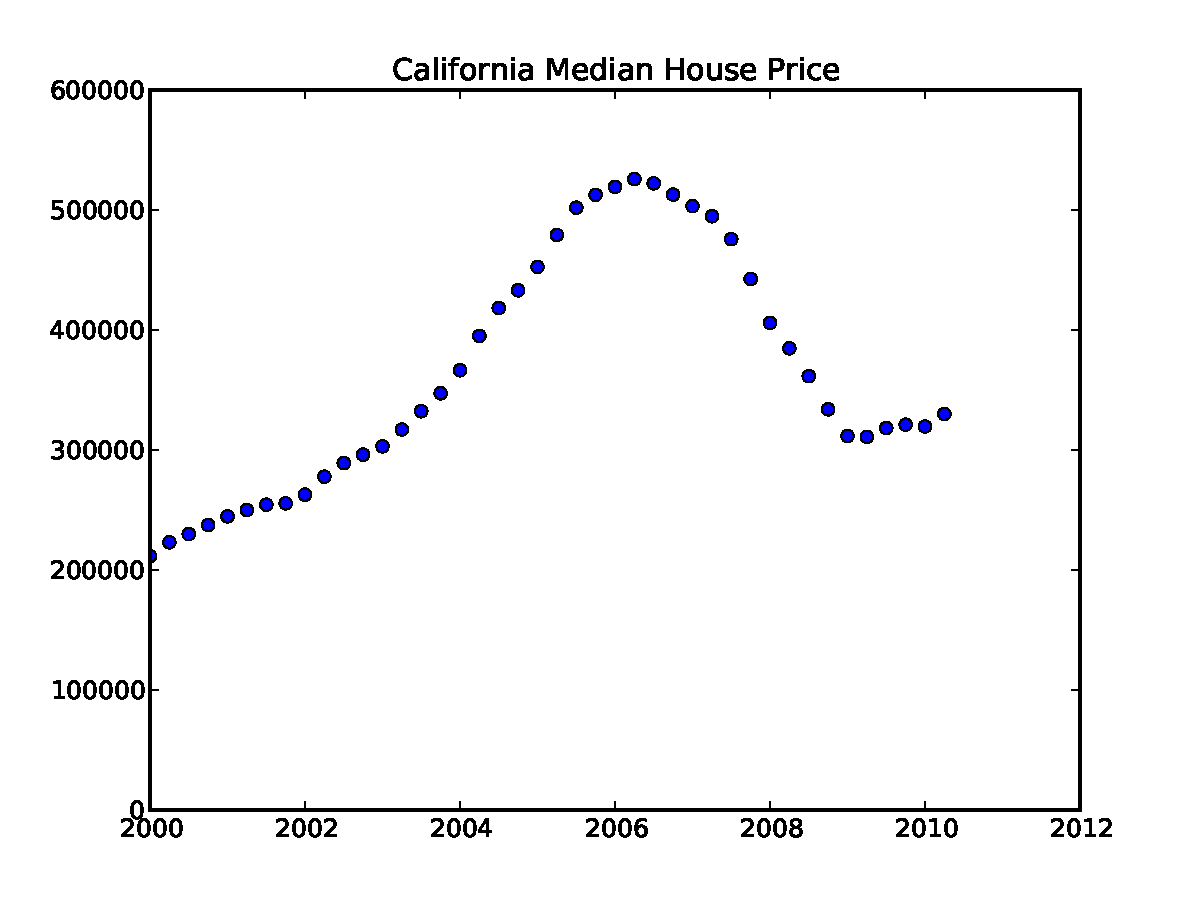
\includegraphics[width=3in]{california.pdf}
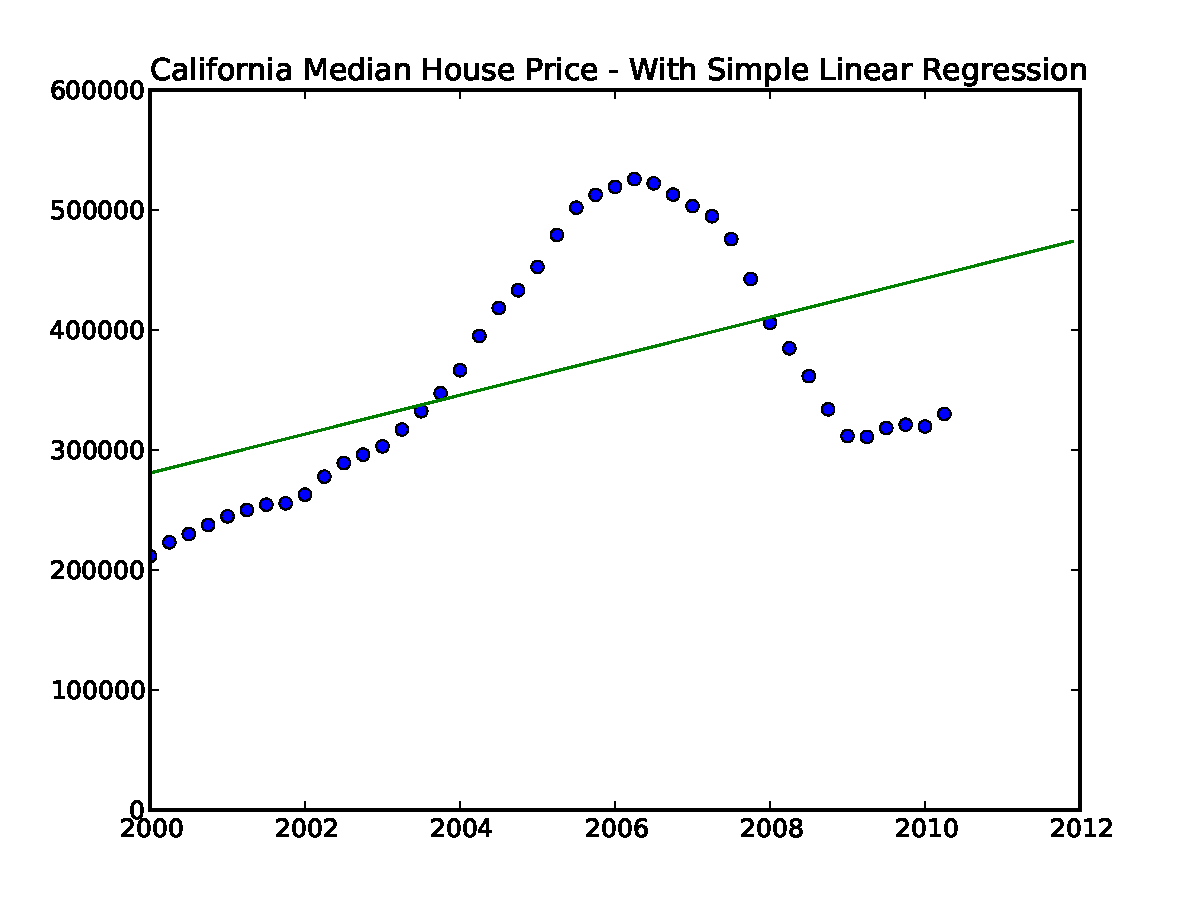
\includegraphics[width=3in]{cali-linear.pdf}
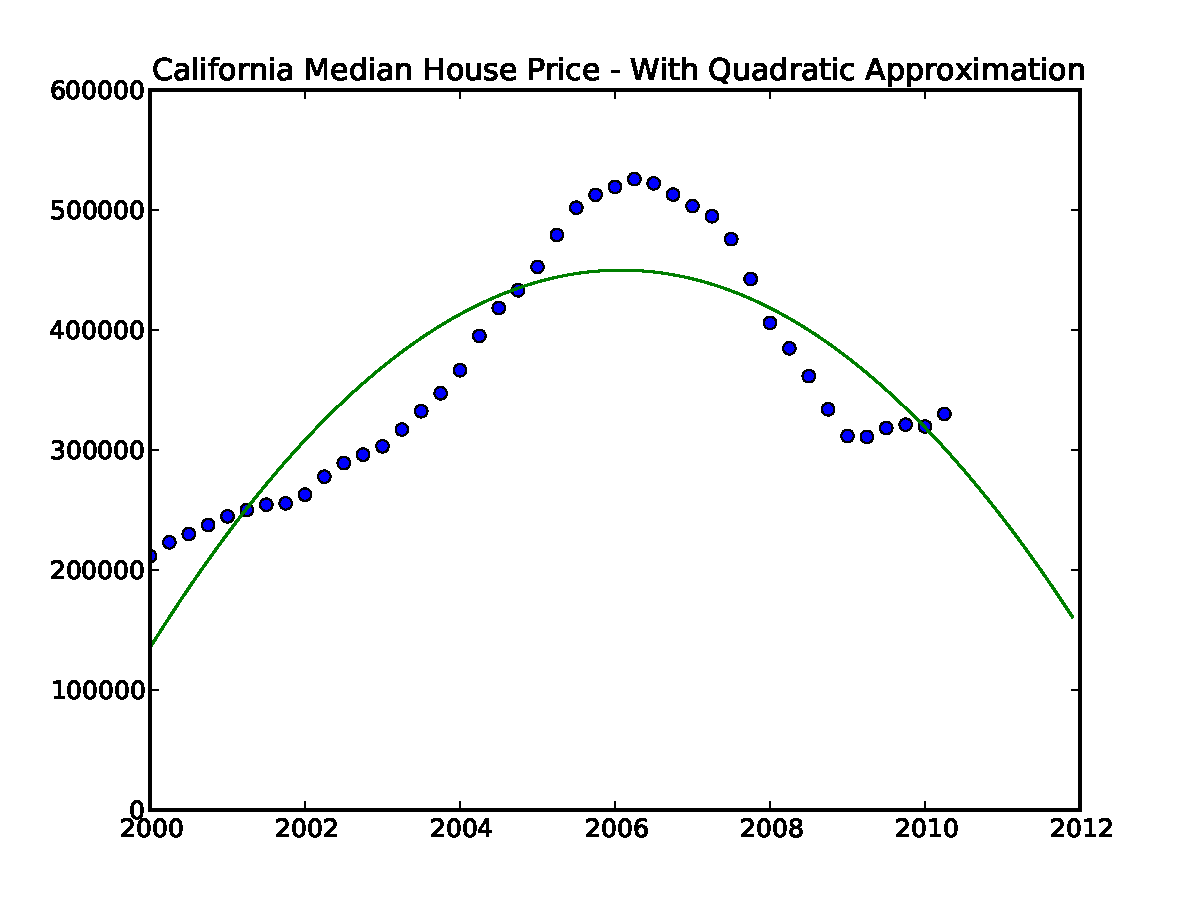
\includegraphics[width=3in]{cali-quadratic.pdf}
\end{figure}

Load the data in housingprices.npy. Note that the years column is years since 2000 (to avoid numerical issues of raising 4 digit numbers to large powers...). 
\begin{problem}
fit cubic. why not great fit? or quartic
\end{problem}


\section*{Logistic Regression}
%Thanks to Wiki, and http://www.statsci.org/data/general/challenger.html 
%http://science.ksc.nasa.gov/shuttle/missions/51-l/docs/rogers-commission/Chapter-4.txt
%Data source: Chatterjee et al (1995). A casebook for a first course in statistics and data analysis. Wiley.
On January 28, 1986, less than two minutes into the Challenger space shuttle's 10th mission, there was a large explosion that originated from the spacecraft. As a result all seven crew members were killed and the shuttle was destroyed. The investigation that followed concluded that the malfunction was caused by damage to O-rings that are used as seals for parts of the rocket engines. There were 24 space shuttle missions before this disaster, and each had 6 primary O-rings. Some of these previous missions noted O-ring damage, but none, obviously, caused this much damage. So what happened? On  the day of the launch, it was $31^{\circ}  \mathbb{F}$, in Florida...

In the dataset "challenger.npy" you'll find data for 23 missions, where the first column is the ambient temperature in Fahrenheit, and the second column is an indicator of the presence of O-ring damage. One of the previous 24 engines was lost at sea, hence 23 data points.  Plotting the points and fitting a cubic curve with linear regression as we discussed above results in the fit shown in Plot----. 

\begin{figure}[h]
\label{badfit}
\centering
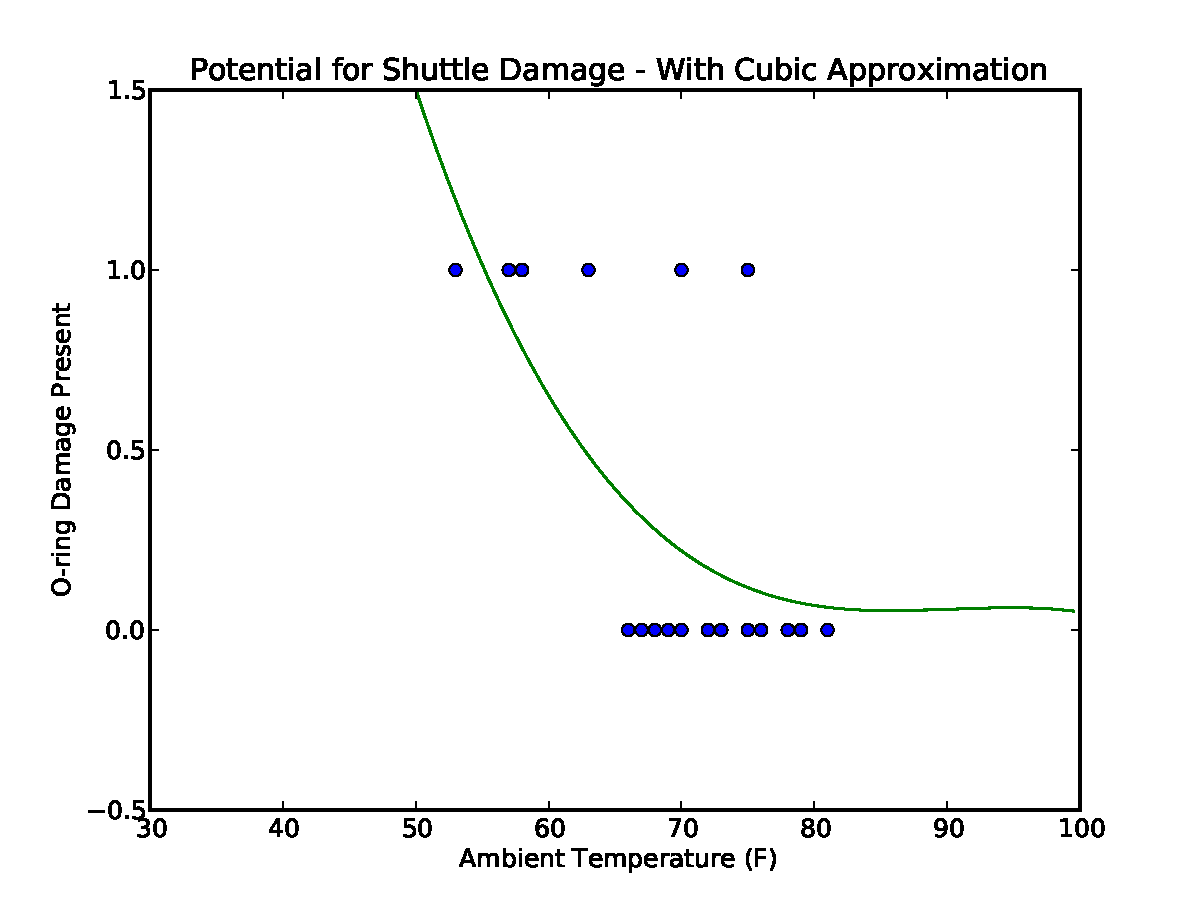
\includegraphics[width=3in]{cubicthrulogitpoints.pdf}
\end{figure}

Clearly, there is a relationship between ambient temperature and O-ring damage. It is also clear that a cubic curve from linear regression is not the ideal model. First and foremost, our response variable (the y axis) is only 0 or 1, based on the presence of damage. ``2" doesn't mean anything, so we shouldn't allow that to occur. In standard linear regression, we assume the $y$ variable follows a normal distribution, as stated previously. However, here we see that our $y$ variable, the presence of O-ring damage, follows a Bernoulli distribution (a Binomial distribution with $n=1$). This is also stated $$y_i \sim Bern(p_i),$$ where $p_i$ is the probability that $y_i=1$, the probability of damage to the O-rings. We see in plot ---- that it appears that $p_i$ is affected by temperature, or in other words, is some function of $x_i$, the ambient temperature.  Thusly, we want to estimate $p_i$ using a linear model, $\underline{x}^T_i \underline{\beta} = \beta_0 + \beta_1x_i$. However, this produces values in $\mathbb{R}$, not just in $(0,1)$. Instead, we model the logit function of the probabilities: 
$$logit(p_i) = log \left(\frac{p_i}{1 - p_i}\right) = \beta_0 + \beta_1x_i,$$ where $logit(p) = log(\frac{p}{1-p}) \in \mathbb{R},$ for $p \in (0,1)$. Furthermore, $$p_i = \frac{e^{\underline{x}^T_i\underline{\beta}}}{1+e^{\underline{x}^T_i\underline{\beta}}}.$$

%This model is shown in Figure ? with arbitrary values for x and y, and $\underline{\beta} = \begin{bmatrix} 0 \\1 \end{matrix}$, such that $p=\frac{e^x}{1+e^x}$. Note the curve shows the estimated probabilities, but the points have only $y=1$ or $0$.

The values of $\beta_0$ and $\beta_1$ would be chosen to minimize $||\underline{y} - \underline{p}||$, for a chosen norm. This can't be solved with the same least squares approach used in linear regression, but instead we look to optimization. This will be introduced later, so for now we'll use a Logistic Regression package in python. 
NumPy has a function sklearn.linear\_model.LogisticRegression that should help.
\begin{verbatim}
from sklearn import linear_model 
model = linear_model.LogisticRegression(C=1000000)
model.fit(X,Y)
\end{verbatim}

Note that X must be a 2-d array or matrix, and by default it automatically includes an intercept. So the vector of temperatures needs to be relabeled/reshaped into a 2-d matrix:

\begin{verbatim}
X=vector_of_temperatures.reshape([23,1])
\end{verbatim}

Once the model has been fit, the slope and intercept of the linear model can be obtained with
\begin{verbatim}
model.intercept_
model.coef_
\end{verbatim} 
and then used to obtain different probabilities of damage given an ambient temperature. This curve is shown below in figure ----. Does it fit better than the cubic polynomial regression?  

\begin{figure}[h]
\label{logisticmodel}
\centering
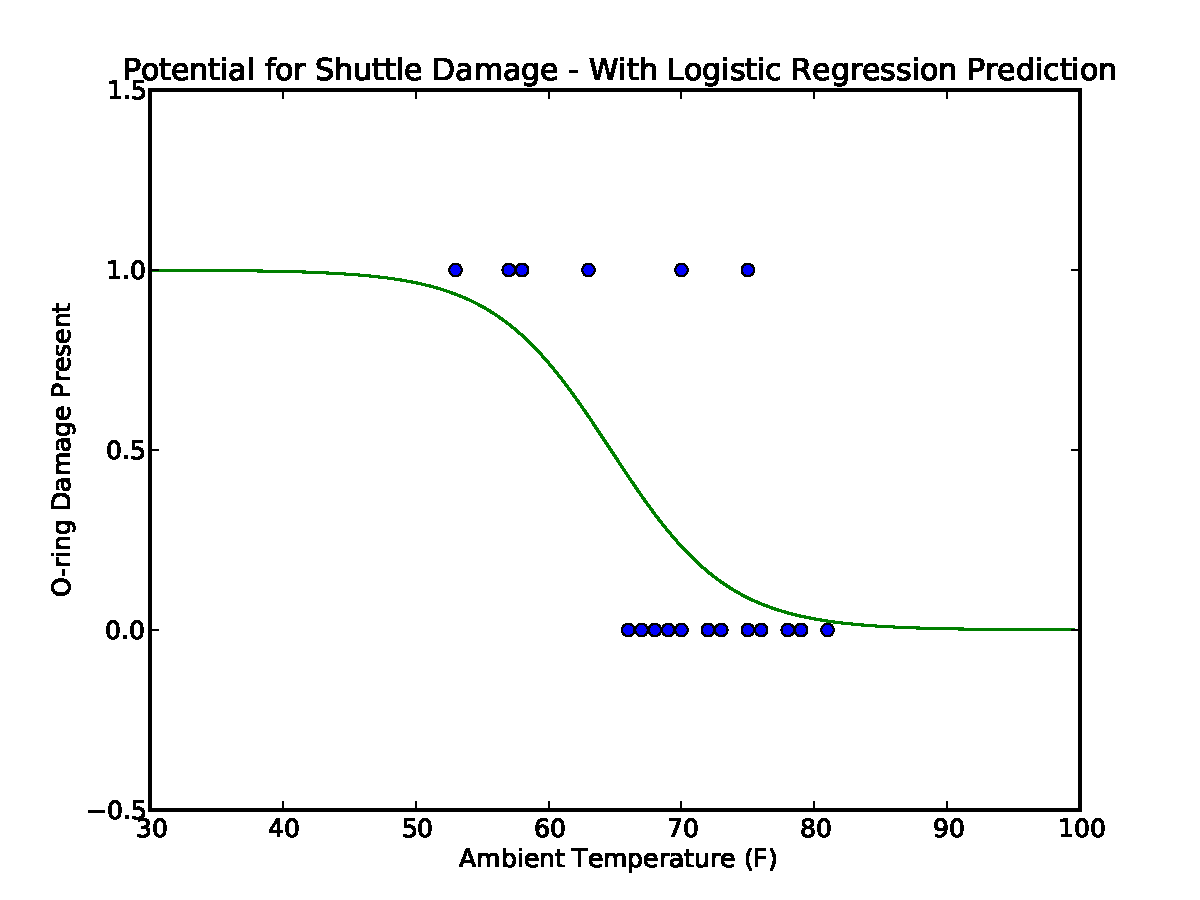
\includegraphics[width=3in]{logreg.pdf}
\end{figure}


\begin{problem}
Run the logistic regression model to predict probability of damage based on ambient temperature, and use it to recreate Figure ---- above. 
\end{problem}

\begin{problem}
Given that it was $31^{\circ}$ F at the time of launch, what was the probability of O-ring damage on January 28, 1986?
\end{problem}
